\chapter{Project Results}
\label{chapter:project_results}
In the following chapter the author is going to analyse the results obtained from the hardware and software developed in this thesis project. The author's first objective was running the \enquote{Hello World!} firmware with the \textit{VexRiscv} \acrshort{cpu}. Secondly, he tested the implementation of the interrupt routine software with the developed \acrshort{clint} hardware. Finally, the candidate successfully executed the minimal Linux \acrshort{os} in real hardware using the developed \acrlong{soc}.

All the results obtained in this thesis which communicate with the \acrshort{fpga} board or the \acrlong{soc} testbench are executing the developed \textit{Console} program. The hardware components comprising the \acrshort{soc} differ in each section of this chapter. The author customizes the \acrlong{soc} hardware depending on the software needs. 

In each step the author studied the simulation with the different logic simulators and the memory resources needed to run the respective firmware. Furthermore, when running the \acrshort{soc} on the \acrshort{fpga} board he examined the required \acrshort{fpga} resources.

\section{System Running \enquote{Hello World!}}
\label{section:hello_world}
The \textit{IObundle} developers created the \enquote{Hello World!} firmware to test the functionality of the \textit{IOb-SoC} template. After the author implemented the \textit{VexRiscv} \acrshort{cpu} on the developed \acrlong{soc}, he executed a regression test to verify the correctness of the \acrlong{soc}. The regression test was the execution of the the \enquote{Hello World!} which was known to work correctly on the \textit{IOb-SoC}.

The \enquote{Hello World!} firmware is a program that prints a \enquote{Hello World!} message to the user, prints the value of $\pi$ which is a floating number and tests file transferring between the \textit{Console} and \textit{IOb-SoC}. The only alteration the author made to the \textit{IOb-SoC} hardware to obtain the results presented in this section was swapping the \acrshort{cpu}.

The \enquote{Hello World!} program size is .... The minimal size of the memory on the \acrlong{soc} is dictated by the firmware size. The memory size should be the closest upper bound power of two.

\subsection{Simulation}
The author simulated the \enquote{Hello World!} program using the \textit{Icarus} simulator and \textit{Verilator}. The \enquote{Hello World!} simulation allows the author to make a fair comparison between both logic simulators. 

In figure \ref{fig:hello_sim} the reader can see the expected output when executing the \enquote{Hello World!} firmware. In this example, the simulator executed the firmware using the internal memory of the \acrlong{soc} and considered that the firmware was already on the memory. Considering the firmware was already on the memory allow the simulator to not execute the firmware transfer between the \textit{Console} and the testbench.

\begin{figure}[!ht]
    \centering
    \begin{subfigure}[b]{0.49\textwidth}
        \centering
        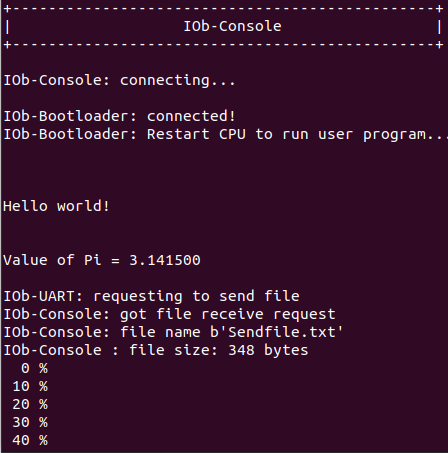
\includegraphics[width=\textwidth]{start_Hello_sim.png}
        \caption{Start of the \enquote{Hello World!} firmware.}
        \label{fig:start_hello_sim}
    \end{subfigure}
    \hfill
    \begin{subfigure}[b]{0.49\textwidth}
        \centering
        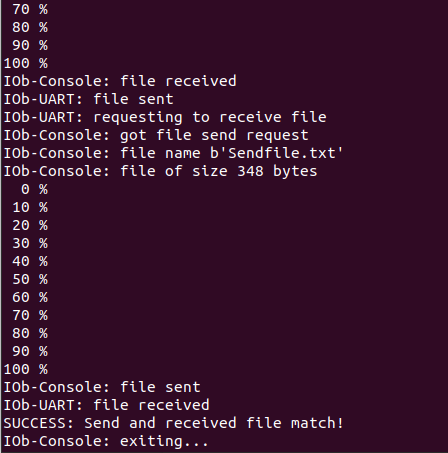
\includegraphics[width=\textwidth]{end_Hello_sim.png}
        \caption{End of the \enquote{Hello World!} firmware.}
        \label{fig:end_hello_sim}
    \end{subfigure}
    \caption{Running Linux with \textit{Verilator}.}
    \label{fig:hello_sim}
\end{figure}

Both open-source logic simulators are capable of executing the \enquote{Hello World!} program. 
% Things that slow the simulation baud rate (serial transfer) and memory access; Baud rate used in simulation was 5000000 which is the number of bits per second transferred to the \acrshort{uart}. The simulations where run considering the system clock frequency 100MHz.

\begin{table}[!ht]
    \centering
    \begin{tabular}{l|ll|ll|}
    \cline{2-5}
                                                           & \multicolumn{2}{l|}{Authors \acrshort{soc}} & \multicolumn{2}{l|}{\textit{IOb-SoC}}    \\ \hline
    \multicolumn{1}{|l|}{Command \textbackslash Simulator} & \multicolumn{1}{l|}{Icarus}  & Verilator & \multicolumn{1}{l|}{Icarus}  & Verilator \\ \hline
    \multicolumn{1}{|l|}{sim-run INIT\_MEM=1}              & \multicolumn{1}{l|}{2m 26s}  & 0m 3s     & \multicolumn{1}{l|}{0m 25s}  & 0m 3s     \\ \hline
    \multicolumn{1}{|l|}{sim-run INIT\_MEM=0}              & \multicolumn{1}{l|}{88m 19s} & 1m 1s     & \multicolumn{1}{l|}{}        & 0m 27s    \\ \hline
    \multicolumn{1}{|l|}{sim-test}                         & \multicolumn{1}{l|}{N/A}     & 2m 27s    & \multicolumn{1}{l|}{43m 34s} & 1m 34s    \\ \hline
    \end{tabular}
\end{table}

From table ... engineers are able to conclude the advantage of using \textit{Verilator}. For more complexed systems the \textit{C++} testbench is much faster than the \textit{Verilog} counterpart. The disadvantage of using \textit{Verilator} is that signal values can only be either '0' or '1'. However, the speed-up in the simulation is also due to the signal value limitation. In \textit{Icarus} the signal are also evaluated as unknown ('x') when they are uninitialized.
% Verilator is slower to compile the testbench; but mush faster executing. The \textit{IOb-SoC} simulation is faster then the authors \acrlong{soc} simulation because the \textit{PicoRV32} is less complex then the \textit{VexRiscv} \acrshort{cpu}.

\subsection{FPGA Board}

fpga-run: 
real	0m41,603s
user	0m0,214s
sys	0m0,119s


\section{Interrupt Routines}

\section{Run/Boot Linux Performance}
\begin{figure}
    \centering
    \begin{subfigure}[b]{0.49\textwidth}
        \centering
        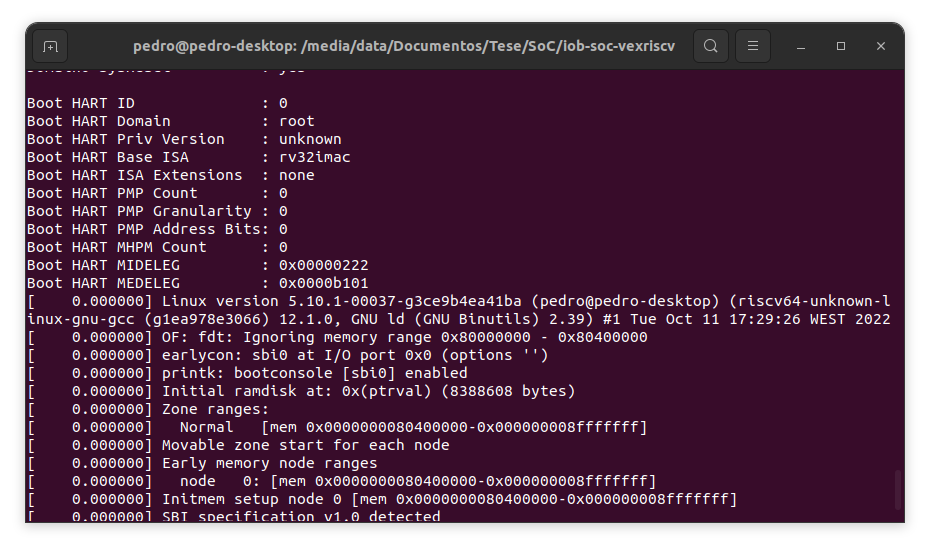
\includegraphics[width=\textwidth]{start_Linux_sim.png}
        \caption{Start of the Linux kernel.}
        \label{fig:start_linux_verilator}
    \end{subfigure}
    \hfill
    \begin{subfigure}[b]{0.49\textwidth}
        \centering
        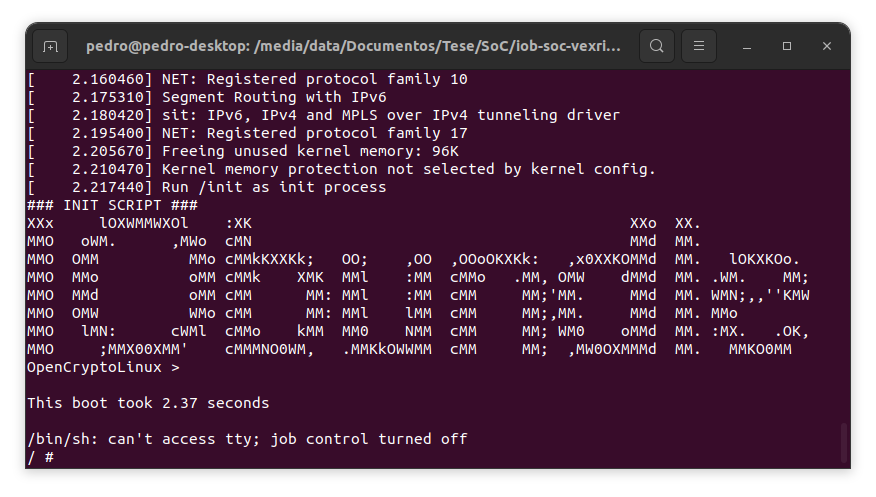
\includegraphics[width=\textwidth]{end_Linux_sim.png}
        \caption{End of Linux kernel boot.}
        \label{fig:end_linux_verilator}
    \end{subfigure}
    \caption{Running Linux with \textit{Verilator}.}
    \label{fig:linux_verilator}
\end{figure}
time that it takes to build a complete OS
real	4m29,570s
user	8m12,039s
sys	0m56,887s

\section{FPGA Resources Consumption}